\documentclass[../main.tex]{subfiles}
\graphicspath{{\subfix{../figures/}}}

\begin{document}
\section{面向对象的基本概念}
\textbf{对象概念的三种观点}
\begin{enumerate}
  \item 从数据结构的角度看,对象是一种\textbf{复杂的数据类型}.
  \item 从软件结构的角度看,对象是一个\textbf{完备的模块},包含了能完成一定功能的函数和局部数据.
  \item 从分析设计的角度看,对象是一个\textbf{活动的实体},可以代表世界的万事万物.
\end{enumerate}
\textbf{对象的内部结构}:对象是一个拥有属性,行为和标志符的实体.
\begin{itemize}
  \item \textbf{属性}:第一种观点:属性也就是变量;第二种观点:属性是程序要处理的数据;第三种观点:描述对象的状态,特征.
  \item \textbf{行为}:第一种观点:行为也就是函数;第二种观点:行为是程序所完成功能的实现;第三种观点:对象具有的改变自身或其他对象状态的活动.
  \item \textbf{标志符}:用于区别对象.
\end{itemize}
\textbf{类的概念}
\begin{itemize}
  \item 类:对一组相似的对象的描述,这一组对象有共同的属性和行为.
  \item 对象与类的关系:对象是类的实例,类是对象的\textbf{模板}.
  \item 同一类的对象,具有不同的属性值,但具有相同的方法.
\end{itemize}
\textbf{方法的类型}
\begin{itemize}
  \item \textbf{属性过程}:对属性的存取操作,维护对象的状态.
  \item \textbf{服务函数}:为其他函数提供服务.比如字符串查找,排序等.
  \item \textbf{接口函数}:类和外界打交道的接口,类通过接口函数为外界提供服务.
  \item \textbf{对象控制函数}:实现对象生命周期的典型功能,控制对象的创建和销毁.
\end{itemize}
\textbf{面向对象系统的基本特征}:
\begin{itemize}
  \item 利用对象进行\textbf{抽象}:主要是提炼相对某种目的的重要的方面,而忽略次要的方面.目的决定了哪些方面是重要的,因此,根据目的的不同,对同一事物可以有不同的抽象.
    是所有程序设计方法的基本工具.自上而下逐步细化,自下而上逐步抽象.
  \item \textbf{封装}:信息隐藏,阻止外界直接对类的状态信息的访问,仅提供方法用以访问和改变它的状态,提高类的安全性.
    提高对象的独立性,有利于灵活地局部修改,提升了程序的可维护性.封装是所有常用的信息系统开发方法的普遍特点.
    传统方法将数据和功能分开封装.面向对象技术则是把功能和数据封装进入对象.
  \item \textbf{消息通信}:
    \begin{itemize}
      \item 是对象协作的灵活机制;模拟现实系统中对象之间的联系;对象之间联系的方法-利用消息进行通信.
      \item 消息:从发送方向接收方发出的执行服务的请求.发送消息通过调用某个类的方法来实现.接收消息通过被其他对象调用本类的方法被实现.
    \end{itemize}
  \item \textbf{生命周期}:设计期-类的生命周期(设计,实现);运行期-对象的生命周期.
    \begin{enumerate}
      \item 对象被创建(调用构造函数,实例化)
      \item 存在
      \item 消亡(区分对象的正常和意外消亡)
    \end{enumerate}
  \item 类层次结构(继承和组合)
  \item \textbf{多态}:
    \begin{enumerate}
      \item 与继承相关的概念,从共同的基类派生出不同的子类,不同子类对象呈现出多种形态。(第三种观点)
      \item 同一对象引用,可以指向不同子类的对象.用父类引用去操作子类对象.(第二种观点)
      \item 方法与对象相关,由对象(具体类型)才能确定方法.(第一种观点)
    \end{enumerate}
\end{itemize}
\textbf{类之间的关联}:描述类之间的关系.
\begin{itemize}
  \item 普通关联(互相独立的类)
  \item 层次结构(互相不独立的类)
    \begin{enumerate}
      \item 整体和部分之间的关系:
        聚合(弱关联关系,部分可有可无,整体和部分可相对独立)和组合(强关联关系,部分不可或缺,整体和部分不可分离)
      \item 泛化/特殊化: 继承.
    \end{enumerate}
\end{itemize}
\textbf{概念之间的关系}:如车辆分为机动车和非机动车. \\
\textbf{继承}:
\begin{itemize}
  \item 体现了类之间的关联关系,该关系把类分成父类和子类.
  \item 代表了概念之间的扩展关系,与人们认知事物的认知过程一致:
  \item 由一般到具体,由模糊到清晰.(第三种观点)
  \item 能够实现某个类无需重新定义就拥有另一个类的某些属性和方法,达到复用和灵活设计的目的,也利于代码的统一维护。(第二种观点)
  \item 子类是父类类型的一种。(第一种观点)
\end{itemize}
\textbf{继承的若干种情况}:
\begin{itemize}
  \item \textbf{一般继承(单继承)}:一个父类拥有一个或多个子类,一个子类只有一个父类.
  \item \textbf{多继承}:一个子类拥有多个父类,描述了现实系统里的概念叠加.多继承可能带来定义冲突,如两个父类具有同名的方法.
    铁锅就是金属和容器这两个概念的叠加.
  \item \textbf{实现式继承}:父类方法只有声明,没有实现.
\end{itemize}
\textbf{继承属性,继承方法}:
\begin{itemize}
  \item 子类具有父类的所有属性.
  \item \textbf{重载(overload)}:在同一个类内部,为同名的方法指定不同的参数表并进行不同的实现.
  \item \textbf{覆盖(override)}:子类为超类的属性和方法指定了新的定义.
\end{itemize}
\textbf{在设计类之间的继承关系时,应注意}:
\begin{itemize}
  \item 用 isa 进行继承关系的测试.
    an A(子类) is a B(父类) (A是一个B)
  \item 父类和子类之间要确实存在继承关系.
    如错误的设计:(父类)猫科动物-(子类)狗
  \item 子类的对象在其生存期内必须保持独特性.
    如错误的设计:(父类)正常用户-(子类)欠费用户
  \item 所有继承下来的特性在每个子类中都必须有意义.
    如错误的设计:车(父类)含属性-油量,汽车(子类),自行车(子类).
\end{itemize}
Example: \textbf{零件管理}:在制造业中,某些类别的复杂产品是由零件装配而成的。常见的需求是记录所有的零件的库存以及这些零件的信息,包括:
\begin{enumerate}
  \item 零件的目录查找号(整数);
  \item 名字(字符串);
  \item 价格(浮点数);
\end{enumerate}
零件可以装配成更复杂的结构,成为组件。一个组件可以包含多个零件,而且可以形成层次结构,即一个组件可以由多个子组件构成,每个子组件又可以由零件或下级子组件构成。

\begin{figure}[H]
  \begin{center}
    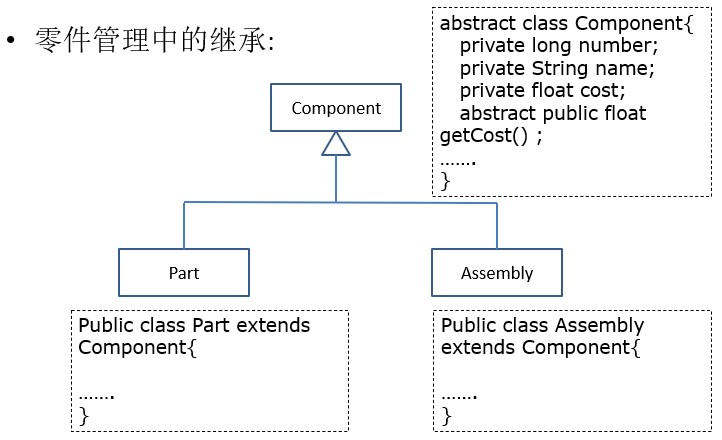
\includegraphics[width=0.50\textwidth]{3_1.jpg}
  \end{center}
\end{figure}
\begin{figure}[H]
  \begin{center}
    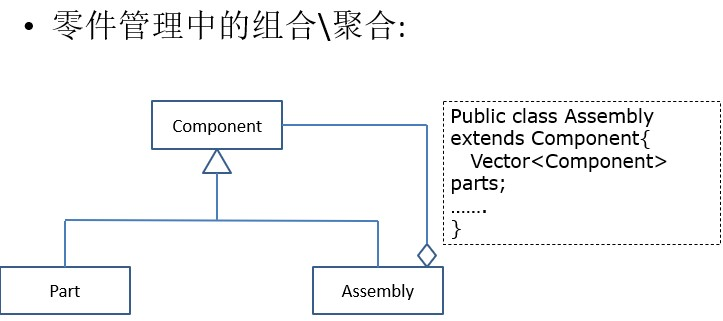
\includegraphics[width=0.50\textwidth]{3_2.jpg}
  \end{center}
\end{figure}
\begin{figure}[H]
  \begin{center}
    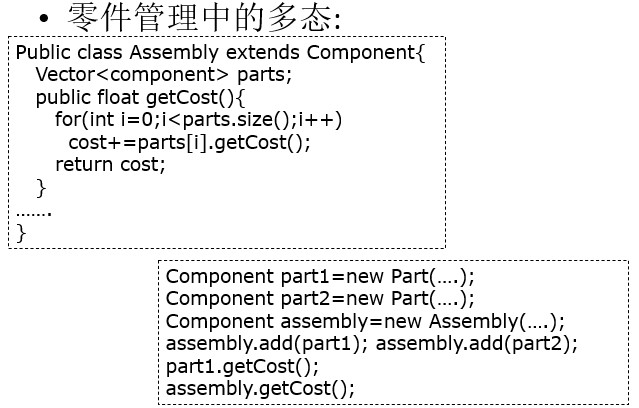
\includegraphics[width=0.50\textwidth]{3_3.jpg}
  \end{center}
\end{figure}

\textbf{继承,重载,多态}:是为了提高系统的灵活性,降低类之间的耦合性.\\
例:在图书馆管理系统中,假设要实现读者借阅图书的功能.对于不同类型的图书(新书,旧书,外文书)有不同的借阅规则(归还日期,费用).请问该如何设计才能提高系统的灵活性(将来可能会增加新的图书类型,该类型可能具有自己特有的借阅规则)

\textbf{抽象类}:描述了系统中的抽象概念.不能实例化的类.通常为子类定义一些公共的接口,指定一些子类必须实现的方法.
\begin{itemize}
  \item 抽象类中有些方法只有声明,没有实现.
  \item 未实现的方法,留给具体类去实现。抽象类只负责定义公共接口.
  \item 抽象类可以具有已实现的方法,因此也具备一般类的继承的优点.
\end{itemize}
\textbf{接口{interface}}:包含属性和抽象方法的特殊的类。接口定义了类之间交流的\textbf{协议}。由硬件接口得名。
接口不能实例化。只能被继承和实现。 \\
\textbf{类,抽象类,接口}三者构成完整的抽象序列机制,描述了人们对系统的认识和理解的过程. \\
\textbf{包}:面向对象技术提供的另一种封装机制.包含了逻辑上功能需要相互协作的类.可用于划分命名空间,解决命名冲突的问题.
可用于划分子系统.

\textbf{可见性}:一个类看到和使用另一个类的资源的能力。
\begin{itemize}
  \item \textbf{公有可见性}:公有属性和方法对整个外界都是可见的。任何其他类都可以访问类的共有属性和方法。
  \item \textbf{私有可见性}:私有属性和方法只对该类的成员可见。
  \item \textbf{保护可见性}:保护属性和方法只对该类和它的子类可见。
  \item \textbf{友类可见性}:友类属性和方法对指定的其他的一些类(友元类)是可见的。
\end{itemize}
\textbf{类属性}:类的所有实例共享的属性.每个类属性只有一个拷贝,无需创建任何类实例,也可以访问这些类属性. \\
\textbf{类方法}:由类定义的方法,只能对类属性进行操作.类方法可以在没有任何类实例的情况下被调用.
\end{document}
